\documentclass[tikz,border=4pt]{standalone}
\usepackage{tikz}
\usetikzlibrary{arrows.meta,positioning,fit,backgrounds,calc}

\begin{document}
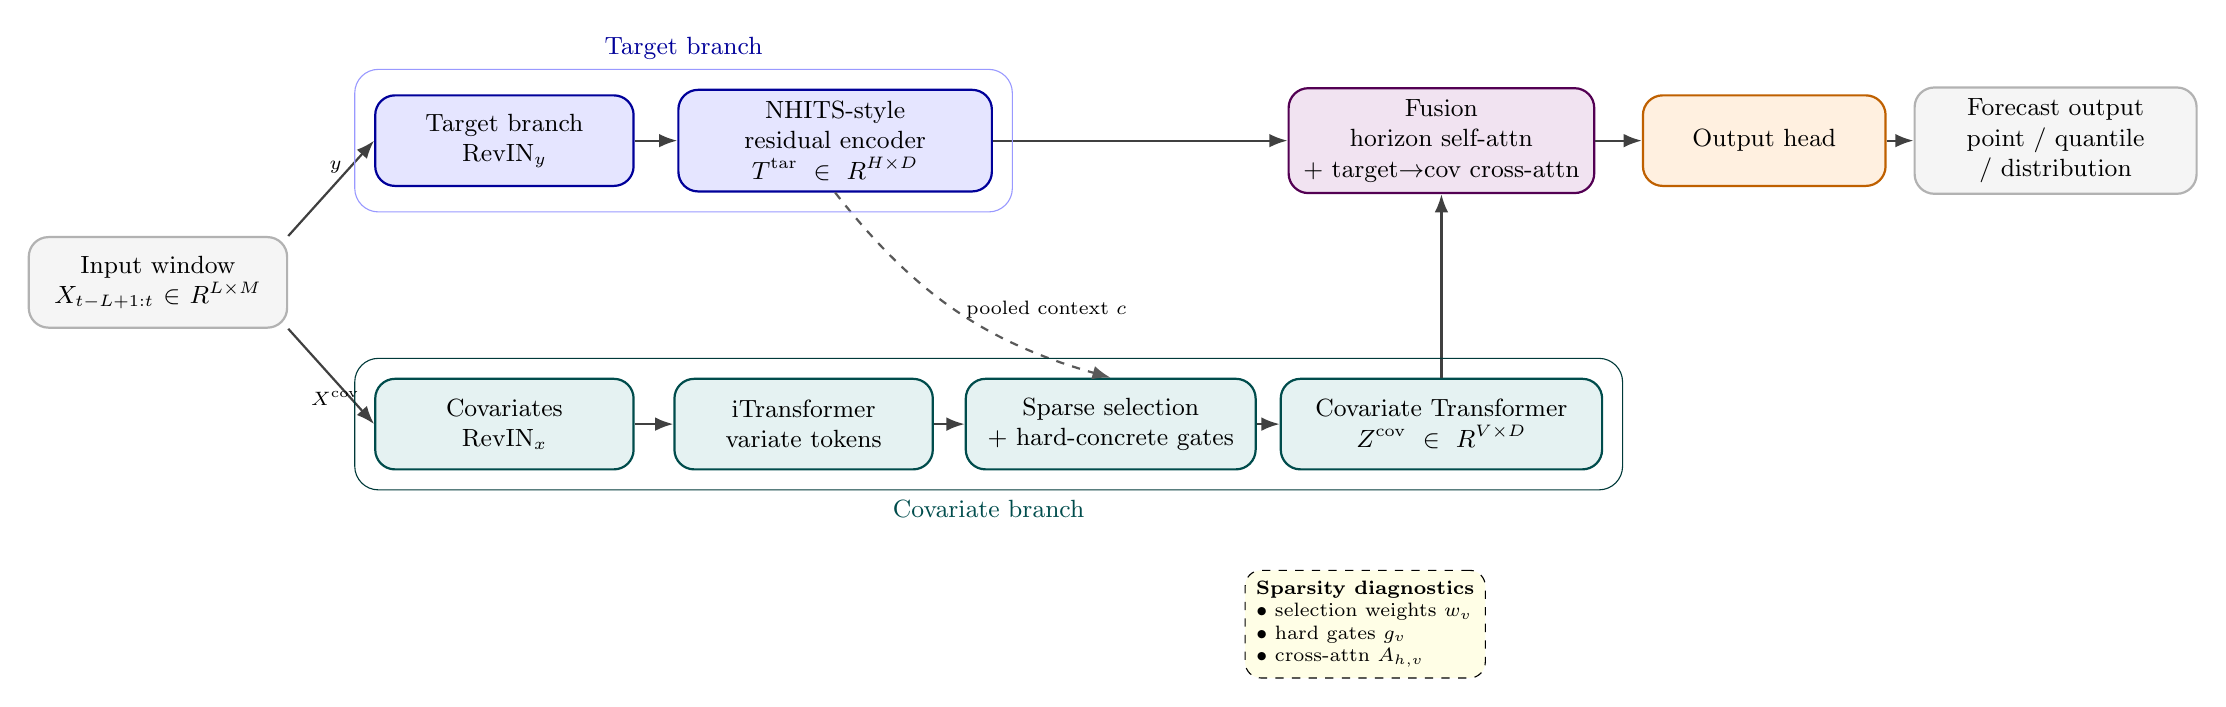
\begin{tikzpicture}[
    x=1cm,y=1cm,
    font=\small,
    >=Latex,
    box/.style={
        draw, thick, rounded corners=2.5mm, align=center,
        minimum height=1.15cm, text width=3.0cm,
        inner sep=4pt, fill=white
    },
    io/.style={box, fill=gray!8, draw=gray!60},
    tar/.style={box, fill=blue!10, draw=blue!60!black},
    cov/.style={box, fill=teal!10, draw=teal!60!black},
    fus/.style={box, fill=violet!11, draw=violet!65!black, text width=3.6cm},
    head/.style={box, fill=orange!12, draw=orange!75!black, text width=2.8cm},
    note/.style={
        draw, dashed, rounded corners=2mm, fill=yellow!10,
        align=left, inner sep=4pt, font=\scriptsize
    },
    arrow/.style={->, thick, draw=black!75},
    darrow/.style={->, thick, dashed, draw=black!65}
]

% Main nodes
\node[io] (input) at (-1,0)
    {Input window\\$X_{t-L+1:t}\in\mathbb{R}^{L\times M}$};

\node[tar] (ty) at (3.4,1.8)
    {Target branch\\RevIN$_y$};

\node[tar, text width=3.7cm] (nhits) at (7.6,1.8)
    {NHITS-style residual encoder\\$T^{\mathrm{tar}}\in\mathbb{R}^{H\times D}$};

\node[cov] (cx) at (3.4,-1.8)
    {Covariates\\RevIN$_x$};

\node[cov] (var) at (7.2,-1.8)
    {iTransformer\\variate tokens};

\node[cov, text width=3.4cm] (sel) at (11.1,-1.8)
    {Sparse selection\\$+$ hard-concrete gates};

\node[cov, text width=3.8cm] (cenc) at (15.3,-1.8)
    {Covariate Transformer\\$Z^{\mathrm{cov}}\in\mathbb{R}^{V\times D}$};

\node[fus] (fusion) at (15.3,1.8)
    {Fusion\\horizon self-attn\\$+$ target$\rightarrow$cov cross-attn};

\node[head] (head) at (19.4,1.8)
    {Output head};

\node[io, text width=3.3cm] (out) at (23.1,1.8)
    {Forecast output\\point / quantile / distribution};

% Arrows from input
\draw[arrow] (input.north east) -- node[pos=0.55, above, font=\scriptsize] {$y$} (ty.west);
\draw[arrow] (input.south east) -- node[pos=0.55, below, font=\scriptsize] {$X^{\mathrm{cov}}$} (cx.west);

% Branch flows
\draw[arrow] (ty) -- (nhits);
\draw[arrow] (cx) -- (var);
\draw[arrow] (var) -- (sel);
\draw[arrow] (sel) -- (cenc);

% Fusion flows
\draw[arrow] (nhits.east) -- (fusion.west);
\draw[arrow] (cenc.north) -- ++(0,0.55) -| (fusion.south);

% Context to selector
\draw[darrow] (nhits.south) to[bend right=18]
    node[midway, right, font=\scriptsize] {pooled context $c$}
    (sel.north);

% Output flow
\draw[arrow] (fusion) -- (head);
\draw[arrow] (head) -- (out);

% Diagnostics note
\node[note, anchor=north west] (diag) at (12.8,-3.65) {\textbf{Sparsity diagnostics}\\
$\bullet$ selection weights $w_v$\\
$\bullet$ hard gates $g_v$\\
$\bullet$ cross-attn $A_{h,v}$};

% Group boxes
\node[
    draw=blue!40, rounded corners=3mm, inner sep=7pt,
    fit=(ty)(nhits),
    label={[blue!60!black,font=\small]above:Target branch}
] {};

\node[
    draw=teal!45!black, rounded corners=3mm, inner sep=7pt,
    fit=(cx)(var)(sel)(cenc),
    label={[teal!60!black,font=\small]below:Covariate branch}
] {};

\end{tikzpicture}

\end{document}